\chapter{Research Methodology}

This chapter will cover research methodology, from the data collection, characterization, categorization, and verification, to analysis.

\section{Background}

Objective
    - find typical patterns in runway incursions
    - identify most frequently occurring runway incursions and causes
    - runway layout
    - conflict geometry
    - cause
    - determine if alert behaviours of industry standard is effective at preventing collisions
    - recommendations

\section{Data Collection}
This project is dependent on the identification of relevant runway incursion incidents that took place globally after 1995. For that, data was collected from databases and reports from various sources. The information provided for each incident and the manner and depth in which said information was conveyed varies across different sources. Thus, there is a need to not only identify the relevant incursions, but to create a data set that presents the information in a way that is useful for browsing, categorization and analysis. For that, the relevant parameters of the incidents were selected, and the data was extracted following a shared standard for all entries in the data set. The parameters that were found to be relevant for this project were the following:

\underline {Runway Geometry:}
Runway geometry refers to the layout of the runway in which the incursion took place. This is dependent on the existence and position of nearby runways. This is important for this project as it describes the location in which the incursion took place. 
\begin{figure}[H]
    \centering
    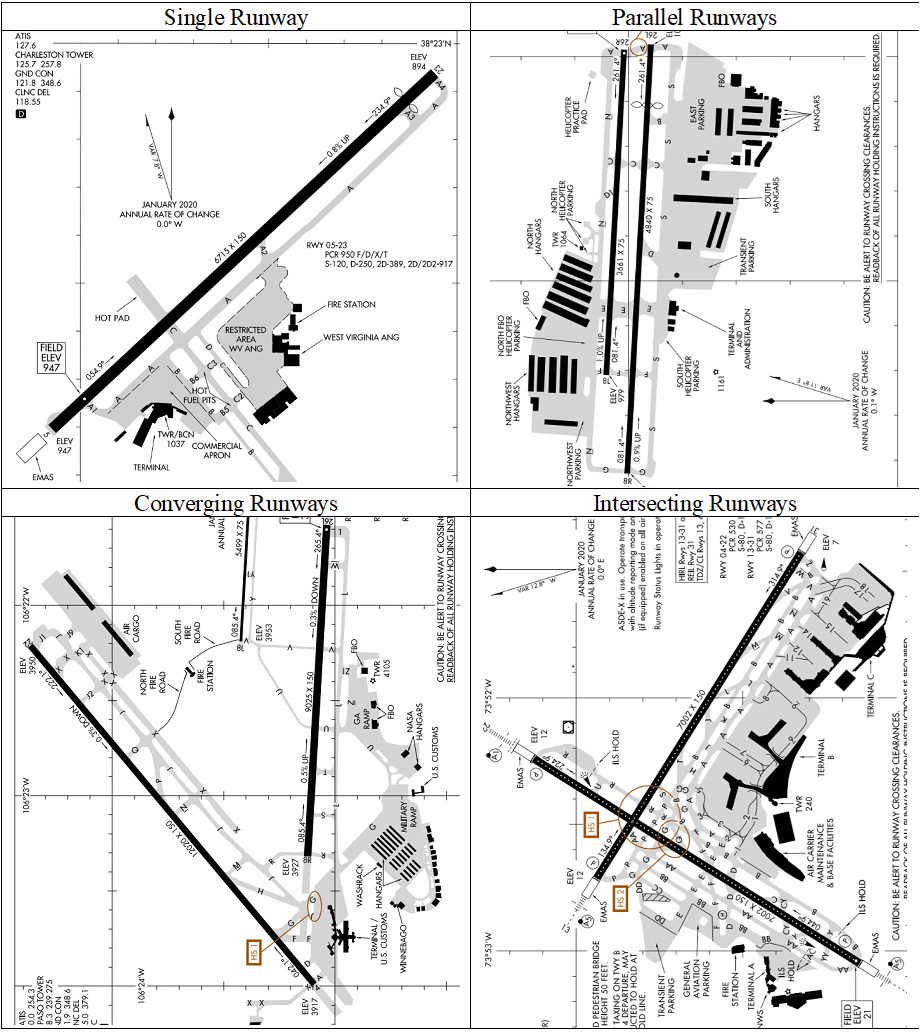
\includegraphics[width = 0.5\textwidth]{Kapitel/runway geometries.png}
    \caption{Runway geometries.}
    \label{fig:enter-label}
\end{figure}

Figure ----- shows 4 types of runway geometries. Single runways are those that do not have any other runway in its vicinity. They can be the only runway in an airport or can be present in airports with multiple runways but with such a separation between them that it can be considered single. Parallel runways are those that run parallel next to each other. Intersecting runways are those that intersect with each other. The angle of the intersection was not considered to be relevant for this project. Converging runways are those that do not physically intersect but whose projections do.

\underline {Type of incident:}
Type of incident describes the cause of the incident by identifying the party at fault. For this project, the type of incidents are differentiated by the following types:

Operational error: An incident caused by the instructions given by the party responsible for ground or aerial traffic control. These incidents can have various causes such as: forgetting previous instructions, failing to communicate instructions, a flawed perception of the current traffic or occupancy of a runway or other human errors.

Pilot deviation: An incident caused when a pilot does not follow instructions, deviates from an approved route and conflicts with other aircraft. These incidents can be caused by poor/lack off communication, confusion or other human errors.

Vehicle deviation: An incident caused by the intrusion of a vehicle in an active runway.

\underline {Class/severity of the incident:}
The classification of the incidents is done by its severity. This is achieved by following ICAO's classification of the severity of runway incursions detailed on ICAO's manual of the prevention of runway incursions. Incursions are classified by severity from A-D, "A" being the most severe. Events with insufficient information are classified as "E". Some of the incidents are assigned an ICAO classification by the entity that does the investigation while others are not. This is mostly dependant on the country in which the incursion took place. If an ICAO severity classification was not given, then one is assigned based on the ICAO classification scheme an the information given in the official report. It is also possible to use the RISC (Runway Incursion Severity Classification) calculator software if there is sufficient information on the incursion.

\begin{figure}[H]
    \centering
    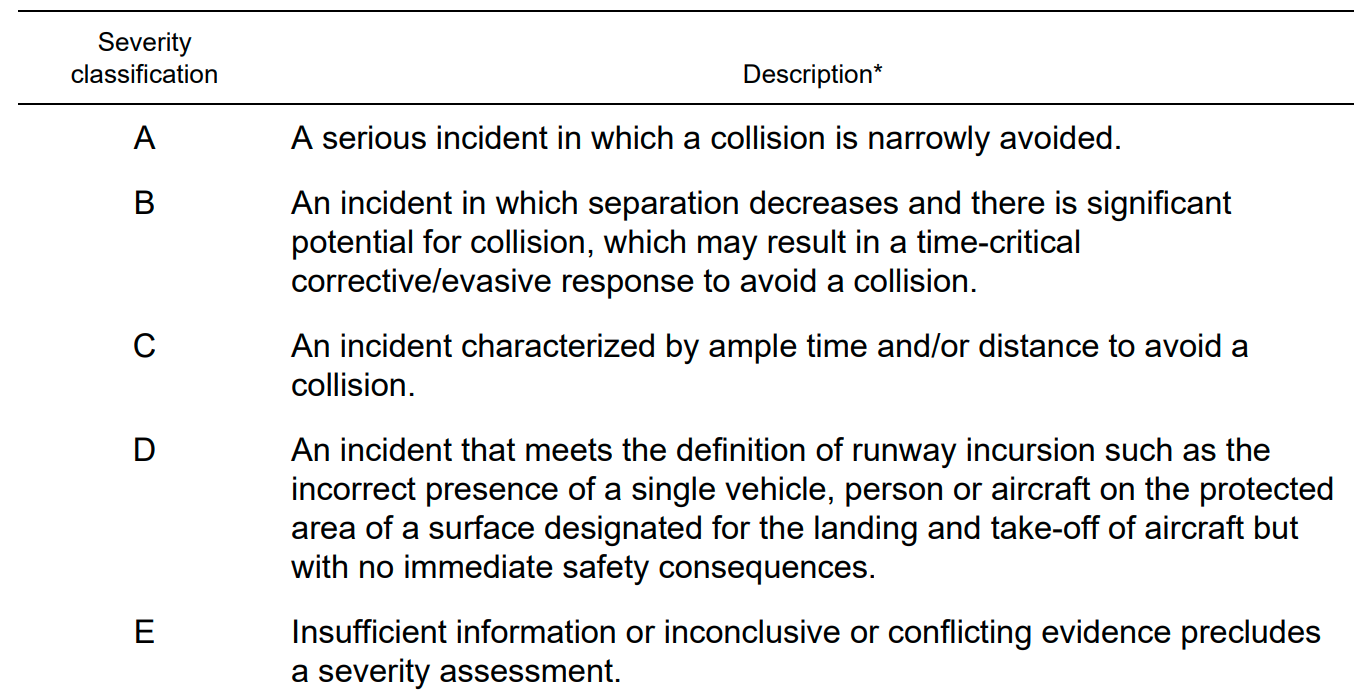
\includegraphics[width = \textwidth]{Kapitel/ICAO Severity classification.png}
    \caption{ICAO runway incursion severity classification scheme}
    \label{fig:enter-label}
\end{figure}

\underline {Model and type of aircrafts involved:} 
This project is mainly concerned with incidents involving commercial or cargo aircrafts. All the incidents that are identified will be added to the data set and they will be categorized by, among other things, the type of aircrafts involved to analyze the incidents.

\underline {OSED states of the aircrafts involved:}
The OSED (Operational Services and Enviromental Definitions) describes the services, functions and procedures for the SURF IA application. It also characterises the enviroment in which it will be used. The OSED states of the aircrafts  derive from this. These OSED States used in DO-323 are the following:

I: Taxiing on Taxiway toward Hold-line or stopped at Holdline.

II: Entering / Crossing / Exiting

III: Takeoff

IV: Approach

V: After Landing

VI: Stopped or taxiing along runway

In the DO-323, These OSED states are used in conjunction with Table A-2 "SURF IA Outputs for all Possible Two-Aircraft State Combinations" to determine which combination of states of the aircrafts involved result in which SURF IA output. In incidents involving pilot deviations, Ownership will be assigned to the aircraft that was following ATC instructions. The aircraft causing the incursion will be the "other aircraft".

\subsection{Sources}
Official websites of organizations investigating aviation accidents and incidents of the following countries were scouted for the reports: Albania, Argentina, Armenia, Australia, Austria, Belgium, Brazil, Bulgaria, Canada, Channel Islands, China, Columbia, Denmark, Estonia, Ethiopia, Finland, France, Germany, Greece, Greenland, Hong Kong, Hungary, Iceland, India, Indonesia, Iran, Italy, Japan, Lithuania, Luxembourg, Malaysia, Mexico, Mongolia, Myanmar, Netherlands, New Zealand, Norway, Peru, Philippines, Poland, Portugal, Republic of Ireland, Russia, Saudi Arabia, Serbia, Singapore, South Africa, South Korea, Spain, Sri Lanka, Sweden, Switzerland, The Bahamas, United Arab Emirates, United Kingdom, United States.

Main and other sources:
\begin{itemize}
    \item FAA Runway incursion database: \url{https://www.asias.faa.gov/apex/f?p=100:5:::NO}
    \item NTSB investigation reports: \url{https://www.ntsb.gov/investigations/AccidentReports/Pages/Reports.aspx}
    \item Aviation Safety Network: \url{https://asn.flightsafety.org/database/}
    \item Bundesstelle für Flugunfalluntersuchung: \url{https://www.bfuweb.de/DE/Publikationen/OpenData/opendata_node.html}
    \item Skybrary: \url{https://skybrary.aero/operational-issues/runway-incursion}
    \item Australia ATSB aviation investigations: \url{https://www.atsb.gov.au/aviation-investigation-reports}
    \item ICAO runway safety statistics: \url{https://www.icao.int/Aerodromes/RunwaySafety/Pages/Statistics.aspx}
\end{itemize}


\subsection{Data Categorization}

After identifying the runway incursions that took place after 1995, extracting the data and adding it to the data set, it is possible to categorize the information to  analyze it and draw useful conclusions. This is a necessary step as not all of the runway incursions that were identified and included in the data set are of part of the main focus of this project. This might because of the type of aircrafts that were involved, the severity of the incident or due to lack of information.

The raw number of incidents identified was 33133, 32898 coming from the FAA. This is because the reporting culture of runway incursion incidents varies from country to country. The FAA lists all of the incidents that are identified, assigns them an ICAO classification and includes them in their database. Other countries don't do this and while reports and investigations are done, it is not done in the same manner as in the United states. That said, severe cases are rare. Events that fit the ICAO classification of "C" and "D" make up the majority of the incursions that take place. To reduce the number of entries that are not the main focus of this project on the data set, FAA incursions of severity "C" and "D" will not be included in the data set. Incursions with incomplete data and those whose cause is listed as "other" will also be omitted. Doing this, the number of runway incursions incidents in the data set is reduced to 484 globally.

\begin{figure}[H]
    \centering
    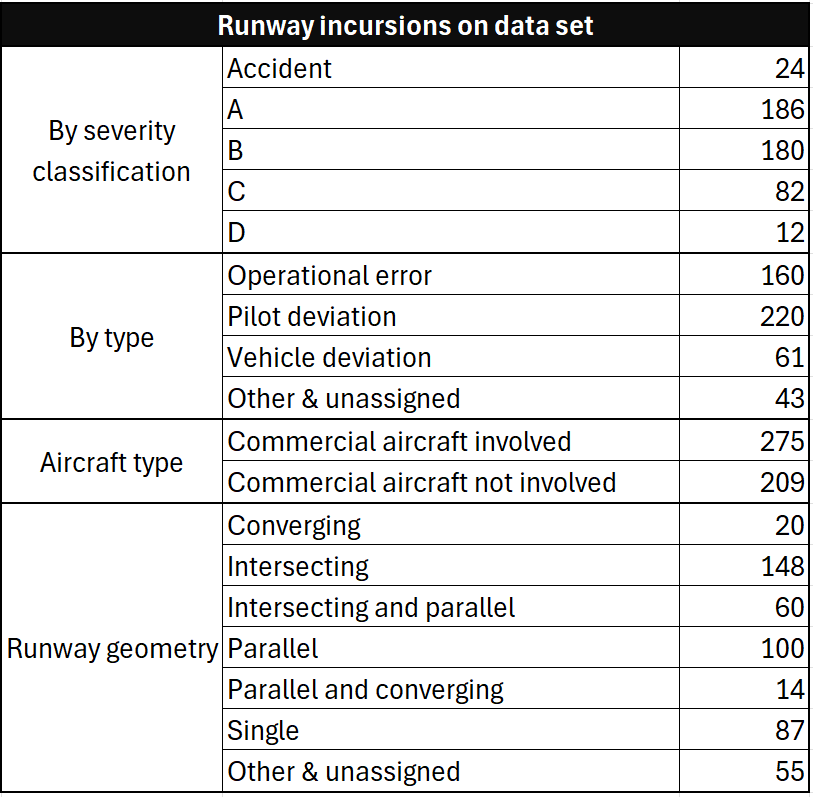
\includegraphics[width = 0.5\textwidth]{Kapitel/Runway incursion full data set classified.png}
    \caption{Classification of data set by different parameters}
    \label{fig:enter-label}
\end{figure}

Figure ---- shows a summary of the full data set. The incidents there are classified by their severity, type, aircraft type and runway geometry. The severity of the incident and the involvement of a commercial aircraft will be used to determine whether the entries are relevant to the main focus of this project.

With the number of entries reduced, the focus shifts to identifying the incidents that are relevant to the main focus of this project, which is severe incidents and accidents involving commercial aircrafts. A distinction will be made between incidents that involve two aircrafts, with at least one of them being commercial, and incidents that involve a ground vehicle and a commercial aircraft. The number of incidents of classification "A" and "B" involving a commercial aircraft is 151. The number of incidents that involve a commercial aircraft and a vehicle is 40. Thus, 191 incidents are found to be relevant for this project.

\subsection{Difference between Data Collected and Data used by SURF IA}

Data collected is conflict geometry, runway geometry, uses severity of outcome based framework. ICAO RIS category based on RISC calculator.

SURF IA uses aircraft states, directionality, speed and calculates a convergence rate to determine if separation will pose safety hazard. In effect, it is calculating a potential collision risk. Uses risk based framework.

to adapt data used, accident reports are read to determine aircraft OSA state in accordance with do323, method of calculating convergence rate is not listed in rtca do 323, just timing thresholds for alerts. 

\subsection{Data Verification}

Collected data severity category was verified using ICAO RISC calculator. faa provides severity levels


\section{Analysis}

\subsection{Alert}